%%% DOCUMENT SETUP %%%
\documentclass[11pt,a4paper]{article}
\usepackage[english]{babel}

%%% LAYOUT %%%
\usepackage{fullpage}
\usepackage[parfill]{parskip}
\usepackage{multicol}
\usepackage{footnote}

%%% GRAPHICS %%%
\usepackage{graphicx}
\usepackage{color}
\usepackage{graphics}
\usepackage{rotating}
\usepackage{subfig}
\usepackage{amsmath}
\usepackage{amssymb}
\usepackage{amscd}
\usepackage{xfrac}
\usepackage{float}
\usepackage{dsfont}

%%% FONT %%%
\usepackage{ifxetex}
\ifxetex
  \usepackage{fontspec}
    \setmainfont{Linux Libertine O}
  \usepackage{xunicode}
  \usepackage{microtype}
\else
  \usepackage[T1]{fontenc}
  \usepackage[latin1]{inputenc}
  \usepackage{times}
  \usepackage{microtype}
\fi

%%% Coding %%%
\usepackage{listings}
\usepackage{pseudocode}

%%% TITLE PAGE %%%
\author{Jeroen Hofman \ \ \ \ \ Carlo Kuiper\\
[15pt] University of Amsterdam (\textsc{UvA})}

\title{Computational Finance\\
  Assignment II: Monte Carlo Methods in Finance.}

\begin{document}
\maketitle
\captionsetup{width=0.8\textwidth}
\graphicspath{{Data/}}
\thispagestyle{empty}

%%% TABLE OF CONTENTS %%%
\newpage
\tableofcontents
\newpage

\section{Part I: Option valuation}
In this part we will compute the option price of an European call and put using Monte Carlo methods. We will compare this to the Black-Scholes value and the results obtained in the previous assignment, where we used a binomial tree to evaluate the option price.

\subsection{Theory}
For determining the price of an option, taking the stock as the underlying, we are interested in the dynamics of the stock price in the market. We start with the Wiener process describing the evolution of the stock price $S$ in a risk neutral world:

\begin{equation}
  \label{eq:ds}
  dS = rSdt + \sigma SdZ
\end{equation}

with $r$ the risk-free rate, $\sigma$ the volatility of the stock and $dZ$ a normally distributed random variable. This process can be discretized dividing the total time $T$ in steps $\Delta t$, so that we can define:

\begin{align}
  N = \frac{T}{\Delta t} \nonumber \\
  S_n = S(n\Delta t)
\end{align}

where $N$ is the total number of steps in the discretization and $S^n$ is the stock price at step $n$. Then, given these equations, we can describe the dynamics of the stock price using the forward Euler method:

\begin{align}
  \label{eq:euler}
  \Delta S &= rS\Delta t + \sigma S\Delta Z \nonumber \\
  S_{n+1} - S_n &= rS_n\Delta t + \sigma S_n\Delta Z \nonumber \\
  &= rS_n\Delta t + \sigma S_n\phi \sqrt{\Delta t} \nonumber \\
  S_{n+1} &= S_n + S_n(r\Delta t + \sigma \phi \sqrt{\Delta t})
\end{align}

where we used that $\Delta Z = \phi \sqrt{\Delta t}$, i.e. the random variation in the stock price over a time $\Delta t$ is a normally distributed function $\phi$ with mean 0 and standard deviation 1 times the square root of $\Delta t$. We introduce an error by discretizing this equation, caused by the truncation of the Taylor expansion which is implicitly used here. 

This scheme is simple and easy to implement in any program, however there is a major downside: it allows for $S_{n+1} < 0$, which is not a physically possible state. The condition for this can be derived as follows:

\begin{align}
  &\frac{S_{n+1}}{S_n} = 1 + r\Delta t + \sigma \phi \sqrt{\Delta t} \nonumber \\
  &\frac{S_{n+1}}{S_n} < 0 \; \text{iff} \nonumber \\
  &\phi < - \frac{1 + r\Delta t}{\sigma \sqrt{\Delta t}}
\end{align}

This condition will occur more often when $r << \sigma$. Luckily we can avoid using equation \ref{eq:euler} since we assume $r$ and $\sigma$ are constant, which allows us to calculate an analytical value. We use equation \ref{eq:ds} and look at the distribution of the log of the stock price, which was also discussed in the previous report, given by:

\begin{align}
  d\text{log}S = (r-\sfrac{1}{2}\sigma^2)dt + \sigma \phi dZ
\end{align}

We can integrate this equation from 0 to T, using that $\int_0^T dZ = Z(T)$, with $Z(T) = \phi \sqrt{T}$ and using explicitly that $r$ and $\sigma$ are constant in time:

\begin{equation}
  \text{log}S_T - \text{log}S_0 = (r - \sfrac{1}{2}\sigma^2)T + \sigma Z
\end{equation}

We can exponentiate this equation to derive at an expression for the stock price at time $T$, given $S_0, r, \sigma$:

\begin{equation}
  \label{eq:st}
  S_T = S_0\text{exp}((r-\sfrac{1}{2}\sigma^2)T + \sigma Z)
\end{equation}

This equation has three advantages over equation \ref{eq:euler}. The first advantage is that it is faster since it only requires one computation (since we are not interested in the stock price at any intermediate time), secondly we cannot get a negative stock price anymore and thirdly we do not have a truncation error using this expression (since it is the analytical solution).

From the calculation of the stock price at time $T$ we can calculate the European call and put option prices $c$ and $p$ as the discounted value of the payoff, where $K$ is the strike price (this has been discussed in more detail in the previous report):

\begin{align}
  \label{eq:optionval}
  c = e^{-rT}\text{payoff} = e^{-rT}\text{max}(S_T - K,0) \nonumber \\
  p = e^{-rT}\text{payoff} = e^{-rT}\text{max}(K - S_T,0)
\end{align}

\subsubsection{MC processes}
In general a Monte Carlo process is a process to approximate an integral which might be too difficult to compute analytically. Suppose we are interested in computing the following n-dimensional integral:

\begin{equation}
  \mu = \int_{a_1}^{b_1} \int_{a_2}^{b_2} ... \int_{a_n}^{b_n} g(x_1,x_2,...,x_n) dx_1 dx_2 ... dx_n
\end{equation}

where $g$ is some continuous function. The key idea is that an estimate of this integral, $\theta$, can be expressed as the expected value of $g$ with as input some random numbers which lie in the intervals on which the integration takes place, i.e.:

\begin{equation}
  \theta = \mathbb{E}g(U_1,U_2,...,U_n)
\end{equation}

where $U_1$ is a uniform random number on $(a_1,b_1)$, $U_2$ is a uniform random number on $(a_2,b_2)$ etc. Furthermore all random numbers are assumed to be independent. Now if we take $k$ sets of ${U_1,U_2,...,U_n}$ then $g(U_1,U_2,...,U_n)$ are all independent and identically distributed random variables with mean $\theta$ and hence we can estimate $\theta$ by:

\begin{equation}
  \theta = \frac{\sum_{i=1}^k g(U_1^i,U_2^i,...,U_n^i)}{k}
\end{equation}

It is important to realize that the estimator $\theta$ itself is a random variable and it can be proven that $\theta$ itself follows a normal distribution using the central limit theorem, given some fixed $k$. Also, by the law of large numbers, the value of $\theta$ converges to the true value $\mu$ (i.e. the exact solution of the integral), when $k \rightarrow \infty$. Since $\theta$ is a random normal variable it is necessary to report an error on the estimate, since $\theta$ may be in one of the tails on the distribution and hence not give an accurate description for $\mu$. The standard error with 95\% confidence intervals on the Monte Carlo estimate $\theta$ is given by:

\begin{equation}
  \label{eq:stderror}
  1.96\frac{\sigma(g)}{\sqrt{k}}
\end{equation}

where $\sigma(g) = \sigma(g(U_1,U_2,...,U_n))$ is the sample standard deviation on the random variables $g(U_1,U_2,...,U_n)$.

\subsection{Method}
We are interested in calculating the price of an option by using the Monte Carlo method as described above. The estimates for an European call and put option price are given by:

\begin{align}
  \label{eq:exppayoff}
  c = e^{-rT}\mathbb{E}[\text{payoff}] = e^{-rT}\mathbb{E}[\text{max}(S_T - K,0)] \nonumber \\
  p = e^{-rT}\mathbb{E}[\text{payoff}] = e^{-rT}\mathbb{E}[\text{max}(K - S_T,0)]
\end{align}

Using equation \ref{eq:st} we simulate a possible path of the stock price, for which we have to use normally distributed random numbers, giving us a value for $S_T$. From this value we can calculate the payoff, either for a call or for a put. We repeat this procedure $M$ times. According to the theory above, the price of the option is then given by:

\begin{equation}
  \label{eq:price}
  c(S_0,t=0) = e^{-rT} \frac{\sum_{m=1}^M\text{payoff}_m (S_T)}{M}
\end{equation}

where $c(S_0,t=0)$ is the MC-estimate of the call option value at time 0, given a stock price at time 0 of $S_0$. The MC estimate also depends on the strike $K$ and the volatility $\sigma$. The error on $c$ is given by $1.96\frac{\sigma(\text{payoff})}{\sqrt{M}}$, where $\sigma(\text{payoff})$ is the sample standard deviation, given by:

\begin{equation}
  \sigma(\text{payoff}) = \sqrt{\mathbb{E}[\text{payoff}^2] - \mathbb{E}[\text{payoff}]^2}
\end{equation}

Note that in this case we know the true value, i.e. the real value of the option $e^{-rT}\mathbb{E}[\text{payoff}]$, since the integral that we are approximating is the evaluation of equation \ref{eq:exppayoff}, giving the Black-Scholes model when analytically solved. Hence we can compare the analytical value with the MC-estimate to validate our model. A second validation would be to check the error which we get. We were able to compute $\mathbb{E}[\text{payoff}^2]$ and hence compute $\sigma(\text{payoff})$ for a call option, so that we can compare the measured MC-error with the analytical expression for the error (see the Appendix, equation \ref{eq:var}).

\subsection{Results}
We wrote a small program that simulates the European call and put option prices using Monte Carlo as described in the Method section above. First we calculate the call and put option prices for $T = 1$, $K = 99$, $r = 0.06$, $S_0 = 100$ and $\sigma = 0.20$. The results are given in table \ref{tab:conv} for sample numbers $M = 10^{5..8}$. The table also gives the Black-Scholes value and the analytical evaluation of the error according to equation \ref{eq:var}. The errors reported are standard errors with 95\% confidence intervals. The Black-Scholes price is 11.544280 for the call option and 4.778969 for the put option.

\begin{table}[H]
  \centering
  \begin{tabular}{l || c | c | c | c | c}
    \hline
    M & Eur. call price & Rel. diff. & Analytical Error & Eur. put price & Rel. diff \\
    \hline
    $10^5$ & 11.537068 $\pm$ 0.100903 & 0.06\% & 0.099330 & 4.779912 $\pm$ 0.052499 & 0.02\% \\
    $10^6$ & 11.530532 $\pm$ 0.031813 & 0.12\% & 0.031411 & 4.764522 $\pm$ 0.016591 & 0.30\% \\
    $10^7$ & 11.548928 $\pm$ 0.010073 & 0.04\% & 0.009933 & 4.773876 $\pm$ 0.005248 & 0.11\% \\
    $10^8$ & 11.545562 $\pm$ 0.003185 & 0.01\% & 0.003141 & 4.778684 $\pm$ 0.001660 & 0.01\% \\
  \end{tabular}
  \caption{Results for the MC-estimate for the European call and put options for different sample sizes as well as the difference with Black-Scholes.}
  \label{tab:conv}
\end{table}

From the table we can directly see the significance of the standard error; while the computed value does not seem to converge strictly to the Black-Scholes value (for example the difference is larger for $M = 10^6$ then for $M = 10^5$), the error becomes smaller if we increase $M$. The Black-Scholes value is within the error range of the values reported in the table for all sample sizes. The fact that the estimate does not seem to converge is caused by the normal distribution of this estimate, as discussed before. However in the limit of $M \rightarrow \infty$ the estimate should still converge to the Black-Scholes value, because the error will converge to 0.

We also see that the errors following from the Monte Carlo distribution are close to the errors computed analytically (with difference in the order of 1\%). This is a second validation for our model and specifically the error analysis that is performed in the model. The analytical error is the error for a perfectly random sample, in this case a random normally distributed sample. So this error is also a measure how well the samples are generated (in this model it is done with the Box-Muller method, see \cite{boxmuller}).

We can compare the standard errors found in table \ref{tab:conv} with the binomial tree model we used in the first assignment. Since the binomial tree model is not a stochastic model the results are fixed for fixed $N$, the number of layers in the binomial tree. Hence it makes sense to compare the error from table \ref{tab:conv} with the difference between the binomial tree method and the Black-Scholes analytical value. We observe an error of 0.001 for $N = 1000$ (11.5453 for the call and 4.7800 for the put), while we need $M = 10^8$ samples to get an error which has the same order of magnitude as the error in the binomial tree. The calculation for the binomial tree took a few seconds in matlab while the computation on $10^8$ samples took around 30 seconds in C. Keeping in mind that matlab is much slower when considering number crunching than C (for the MC method it is a factor 120 slower), the MC method is computationally very expensive compared to the binomial tree method.

Next we consider the option price as a function of the strike price $K$. We vary $K$ between 0 and 200 and calculate the MC estimate over $10^6$ samples for each value of $K$. Figure \ref{fig:strike} below shows the value of the put (red) and the call (blue) option on the left side, and the corresponding errors on the right side. From the left figure we see some familiar behavior, if the strike becomes higher, the call option value decreases and the put option value increases because the payoff becomes less and more respectively, and hence this will also be the case for the expectation of the payoff. However if we observe the error we see some interesting behavior; if the corresponding option price goes to zero the error also goes to zero. When the option price increases, the error also increases but it becomes constant. This can be explained by looking at the individual measurements of the payoff. Consider the put option, if the strike becomes lower, the payoff will hit the lowest possible value of 0 more often and hence the sample will consists of a bunch of zeros and some values slightly larger than zero, this will cause the error to drop, since many measurements have the same value. If the strike increases, this effect will disappear because the 0 is sampled less and the error will become independent of the strike price since 0 is not being sampled significantly anymore. The error would have been strike price independent at 0.042 (in the figure) if the payoff would not have a minimum zero, but would instead be unbounded with payoff $S_T - K$ or $K - S_T$.

\begin{figure}[H]
  \centering
  \subfloat{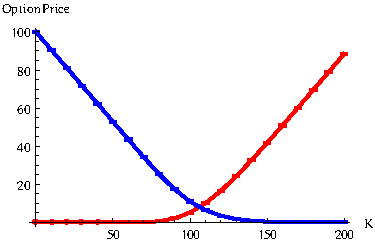
\includegraphics[width=0.4\textwidth]{strike.pdf}}
  \subfloat{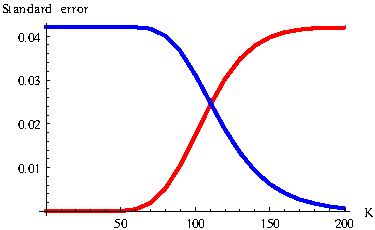
\includegraphics[width=0.4\textwidth]{strikeerror.pdf}}
  \caption{The put (red) and call (blue) option prices as a function of $K$ (left figure) and the error as a function of $K$ (right figure).}
  \label{fig:strike}
\end{figure}

Another way to look at this is that the Monte Carlo dynamics assume that the estimate is a normally distributed random variable. If the error would not converge to zero, one could have a MC-estimate with a mean close to zero but with a standard error which is larger than the distance between the mean and 0. This would imply that repeated measurements of the MC-estimates could generate values lower than zero (since they lie within the standard error) but this can obviously not be the case as the lowest possible estimate is 0 (if all the samples have 0 payoff for a certain measurement). Hence the standard error has to converge to zero if the option price converges to zero to satisfy the central limit theorem.

Of course even if the error goes to zero if the option price does so there is still a finite probability that our MC-estimate would be smaller than zero if we assume the MC-estimate to be perfectly normally distributed. However in our measurements this would suggest we need to sample a value more than 40 $\sigma$ away from the mean, the probability of sampling such a value is very small ($10^{-350}$) so it is save to assume we would not sample such a value.

We can repeat the same measurements, but varying the volatility instead of the strike price. Figure \ref{fig:vol} shows the put option price (red) and the call option price (blue) as a function of the volatility (measured from 0 to 1 in steps of 0.05). The other parameters are $S_0 = 100, K = 99, r = 0.06$ and $M = 10^6$. The figure shows again the error as a function of the volatility.

\begin{figure}[H]
  \centering
  \subfloat{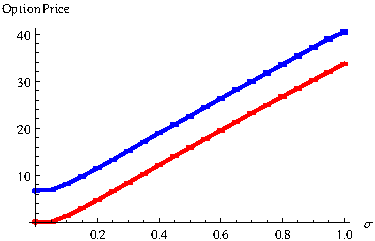
\includegraphics[width=0.4\textwidth]{vol.pdf}}
  \subfloat{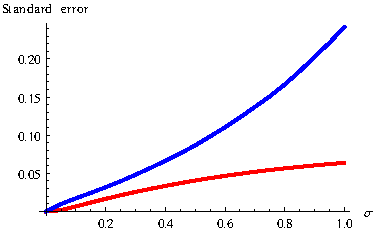
\includegraphics[width=0.4\textwidth]{volerror.pdf}}
  \caption{The put (red) and call (blue) option prices as a function of $\sigma$ (left figure) and the error as a function of $\sigma$ (right figure).}
  \label{fig:vol}
\end{figure}

We see from the left figure that if the $\sigma = 0$, the call option is still worth $(S_0*\text{exp}(0.06) - K) * \text{exp}(-0.06)$ because of the drift in the stock price (the random term is 0) given by the risk-free interest rate, while the put option is worth nothing because $K < S_T$ and hence the payoff is always zero. If the volatility is increased the option prices increase linearly for both options because the loss for a price drop (for a call) and a price rise (for a put) is almost constant while the profit for a price rise (for a call) and a price drop (for a put) does increase, so both option types benefit from an increased volatility in the market. The exact increase can be calculated precisely with vega from the Black Scholes model: $\nu=\partial C/ \partial \sigma$ and it matches the left figure exactly in the plot below.

\begin{figure}[H]
  \centering
  \subfloat{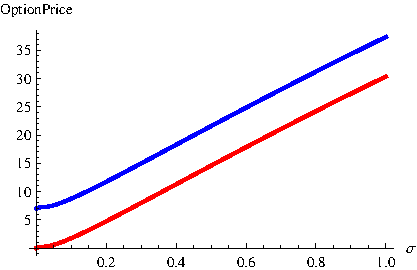
\includegraphics[width=0.4\textwidth]{Vega.pdf}}
  \caption{The put (red) and call (blue) option prices as a function of $\sigma$ calculated analytically with vega.}
  \label{fig:vega}
\end{figure}

If we look at the errors we would expect beforehand the errors to scale linear with $\sigma$ because it is a measure of the spread in option prices (and hence in payoff), however this is not the case. We observe a super-linear increase of the error for a call and a sub-linear increase for a put. This is caused by a difference in values for the put and call payoff. By equation \ref{eq:st} the stock price at maturity is always positive, this means that the payoff for a put can be at most $K$ (and at least 0). The payoff for a call however is in theory unbounded, the payoff can be anywhere from 0 to $\infty$. The larger range of different payoffs (hence different samples) which can occur for a call option compared to a put option, gives a higher standard-deviation and hence a larger error for the call then for the put option price. This effect becomes more visible when $\sigma$ is large, which generates larger payoffs, and hence the upper bound for the put becomes important. In fact, when $\sigma \rightarrow \infty$, the standard deviation of the put option would still be finite (because the payoff is then either 0 or $K$), but the standard deviation of the call option will not be (because it is either 0 or $\infty$).

\newpage

\section{Part II: Sensitivity Analysis}
In this part we calculate the hedge parameter $\delta$ for a Monte-Carlo simulation using finite differencing and the likelihood-ratio method. We calculate $\delta$ both for an European call as well as a digital call option and we investigate the accuracy as a function of sample size and perturbation size.

\subsection{Theory}

In previously studied Black-Scholes model it was straightforward to calculate the value of the hedge parameter $\Delta$, the value of the option $V$ at time $T$ differentiated to the current stock price $S$, defined by:

\begin{equation}
  \label{eq:delta}
  \Delta = \frac{\partial V}{\partial S}
\end{equation}

However $\Delta$ cannot always be derived easily in other models or for more exotic options. Three methods are generally used for estimating $\delta$: bump-and-revalue methods, likelihood ratio methods and path-wise differentiation methods. All three methods are described in Glasserman \cite{Glasserman}. Path-wise differentiation methods fall outside the scope of this assignment. These methods are more general, in the sense that they can approximate any the derivative of a function $f(\theta_0,...,\theta_n)$ with respect to some parameter $\theta_i$, we name this partial derivative $\alpha_i$.

\begin{equation}
  \alpha_i(\theta_0,...,\theta_n) = \frac{\partial f(\theta_0,...,\theta_n)}{\partial \theta_i} \; \text{ where } 0 \leq i \leq n
\end{equation}

In our case of estimating $\Delta$, we choose $i$ such that $\theta_i=S$ and set $f(\theta_0,...,\theta_n)$ equal to the option value $V(S)$, so that $\Delta$ becomes $\alpha_i(\theta_0,...,\theta_n)$.

In a bump-and-revalue method the same simulation for $f$ is used with different parameters to estimate $\delta$. The simplest method uses the forward Euler method. We apply the forward difference method with a perturbation $\epsilon$. So we look at the Taylor expansion of $f(\theta_i+\epsilon)=f(\theta_0,\ldots,\theta_i+\epsilon,\ldots,\theta_n)$ around $f(\theta_i)=f(\theta_0,\ldots,\theta_i,\ldots,\theta_n)$

\begin{equation}
f(\theta_i+\epsilon)=f(\theta_i)+\alpha_i(\theta_0,...,\theta_n)\epsilon+\frac{\partial^2 f(\theta_i)}{\partial \theta_i^2}\epsilon^2+\ldots
\end{equation}

and then obtain the forward difference estimating $\alpha_i(\theta_0,...,\theta_n)$ by ignoring terms with $\epsilon^2$ higher. The (truncation) error that will arise is of the order $\epsilon$

\begin{equation}
  \alpha_i(\theta_0,...,\theta_n) \approx \frac{f(\theta_i + \epsilon) - f(\theta_n)}{\epsilon}
\end{equation}

It is a rough approximation and it can be shown that it is not very stable (as we will see with the digital option later on) as well as having only $\mathcal{O}(\epsilon)$ accuracy, since we ignore the $\epsilon^2$ term in the Taylor expansion. We can also apply another bump-and-revalue method known as central differencing to get a smaller error, it has $\mathcal{O}(\epsilon^2)$ accuracy. However, this method does require an extra evaluation, namely $f(\theta_i-\epsilon)=f(\theta_0,\ldots,\theta_i-\epsilon,\ldots,\theta_n)$. When we subtract the Taylor expansions of $f(\theta_i-\epsilon)$ from $f(\theta_i+\epsilon)$  (both Taylor expansions are around $f(\theta_i)$), we get

\begin{equation}
f(\theta_i+\epsilon)-f(\theta_i-\epsilon)=2~\alpha_i(\theta_0,...,\theta_n)~\epsilon + \frac{2}{3!}\frac{\partial^3f(\theta_i)}{\partial \theta_i^3}\epsilon^3+\ldots
\end{equation}

and then obtain the central difference estimating $\alpha_i(\theta_0,...,\theta_n)$ by ignoring the terms with $\epsilon^3$ or higher. The (truncation) error that arises is of the order $\epsilon^2$.

\begin{equation}
\label{eq:cd}
\alpha_i(\theta_0,...,\theta_n) \approx \frac{f(\theta_i + \epsilon) - f(\theta_i - \epsilon)}{2\epsilon}
\end{equation}

More information on the central difference method can be found in \cite{heath}. We will apply these formulas directly to equation \ref{eq:delta} to obtain forward and central differencing formulas for the case of the hedge parameter $\Delta$. But first we will study a different refined method: the likelihood ratio method. 

For this method we need to introduce some terminology. Let $\theta$ be the current stock price, $S_T$ be the stock price at time $T$, $f(S_T)$ the payoff at time $T$ from the option, $g(S_T,\theta)$ the probability density function of $S_T$ with initial stock price $\theta$ and $V(\theta)=\mathbb{E}[f(S_T)]$ the expected payoff of the option. Now we can start with the calculation off $\Delta$.

\begin{align}
\Delta=\frac{\partial V(\theta)}{\partial \theta}&=\frac{\partial \mathbb{E}[f(S_T)]}{\partial \theta}\\
&=\frac{\partial \int f(S_T)g(S_T,\theta)\mathrm{d}S_T}{\partial \theta}\\
&\stackrel{*}{=}\int f(S_T) \frac{g(S_T,\theta)}{\partial \theta} \mathrm{d}S_T\\
&=\int f(S_T) \frac{\dot{g}(S_T,\theta)}{g(S_T,\theta)} g(S_T,\theta) \mathrm{d}S_T\\
&=\mathbb{E}\left[f(S_T) \frac{\dot{g}(S_T,\theta)}{g(S_T,\theta)}\right]\\
\end{align}

At $\stackrel{*}{=}$ we move the partial derivative into the integral. To do this we need to have a payoff that is smooth and differentiable almost everywhere (\cite{savickas}).

The idea behind the likelihood ratio method is to estimate $\mathbb{E}\left[f(S_T) \frac{\dot{g}(S_T,\theta)}{g(S_T,\theta)}\right]$ which is equal to $\Delta$. We found out that for this method to work the payoff has to be smooth and differentiable almost everywhere.

We are going to use the likelihood ratio method for a digital option. The payoff $f(S_T)=I\left\{S_T>K\right\}$ is indeed smooth and differentiable, so it can be used. The strategy is to calculate a nice expression of $f(S_T) \frac{\dot{g}(S_T,\theta)}{g(S_T,\theta)}$ and then with Monte Carlo simulation obtain an estimate of the expected value. Without loss of generality we can assume that the current stock price is the stock price at time $0$. For the digital option a lot a lot of terminology is required:

\begin{align}
&S_T=\theta e^{(r-\sigma^2/2)T+\sigma\sqrt{T}Z} \text{   denotes the stock price}\\
&g(S_T,\theta) \text{   is the distribution of the lognormal distributed $S_T$}\\
&g(S_T,\theta)=\frac{1}{S_T\sigma\sqrt{T}}\phi(\xi(S_T,\theta)) &\\ &\xi(S_T,\theta)=\frac{\log\frac{S_T}{\theta}+(r-\sigma^2/2)T}{\sigma\sqrt{T}} &\\
\end{align}

With a little bit of calculus we get $\frac{\partial g(S_T,\theta)}{\partial \theta}=\dot{g}(S_T,\theta)=\frac{1}{S_T\sigma\sqrt{T}}-\xi(S_T,\theta)\phi(\xi(S_T,\theta))\frac{1}{\theta\sigma\sqrt{T}}$

Then the final calculation comes down to, we substitute $S_T$ for $\theta e^{(r-\sigma^2/2)T+\sigma\sqrt{T}Z}$,

\begin{equation}
f(S_T) \frac{\dot{g}(S_T,\theta)}{g(S_T,\theta)}=I\left\{S_T>K\right\}\frac{\sigma\sqrt{T}Z}{\theta\sigma^2T}=I\left\{S_T>K\right\}\frac{Z}{\theta\sigma\sqrt{T}}
\end{equation}

Apply Monte Carlo simulation to get an estimation for the expected value

\begin{equation}
\label{eq:likeli}
\Delta=\mathbb{E}\left[f(S_T) \frac{\dot{g}(S_T,\theta)}{g(S_T,\theta)}\right]\approx\frac{1}{n}\sum_{i=1}^n e^{-rT}I\left\{S^i_T>K\right\}\frac{Z^i}{\theta\sigma\sqrt{T}}
\end{equation}

\subsection{Method}
We will first describe the method for calculating $\delta$ in case of an European call. Using the theory described above we can calculate the value for $\delta$ as follows: We first compute an MC-estimate of an European call option $C(S_0)$ (the bumped value, equation \ref{eq:price}) given initial stock price $S_0$, then we generate another MC-estimate $C(S_0 + \epsilon)$ (the unbumped value) given an initial stock price $S_0 + \epsilon$, we do this by generating stock prices according to equation \ref{eq:st} and then calculating the payoff, as in Part I. Then we apply forward differencing to calculate $\delta$:

\begin{equation}
  \label{eq:deltabumped}
  \delta \approx \frac{C(S_0 + \epsilon) - C(S_0)}{\epsilon}
\end{equation}

Both MC-estimates have a sample variance (and hence an error), it is straightforward to derive that:

\begin{equation}
  \text{Var}(\delta) = \frac{\text{Var}(C(S_0+\epsilon)) + \text{Var}(C(S_0)) - 2\text{Cov}(C(S_0),C(S_0 + \epsilon))}{\epsilon^2}
\end{equation}

If both MC-estimates are sampled with different seeds, the covariance will be 0 (if the samples are truly random) and the error will be much larger then when both samples are generated with the same seed, when they will be positively correlated because of the use of the same set of random numbers. We will do both simulations, one where both estimates have the same random seed and one where both have different seeds. We see from the variance that the error will blow up in the limit of $\epsilon \rightarrow 0$, provided the relative difference between the variances and covariance converges slower than $\mathcal{O}(\epsilon^2)$. It is important to note that $\delta$ is an MC-estimate as well, since it is the difference of two MC-estimates, hence it also follows an underlying distribution with mean $\mu = \frac{\text{BS}(S_0 + \epsilon) - \text{BS}(S_0)}{\epsilon}$ and variance $\mathbb{E}[\sigma^2]$, with $\sigma^2$ as given above.

For the digital option we also apply formula \ref{eq:deltabumped} where $C(S_0)$ is now the Monte-Carlo estimate of the payoff for a digital option $I{(S_T > K)}$, i.e. 1 when the stock price at maturity is higher than the strike, 0 otherwise. Next to this implementation we also use the central difference scheme to calculate the Monte-Carlo estimate, given by equation \ref{eq:cd} which is implemented in the same way. In both methods we will use the same seeds for the Monte Carlo estimate as the next section will show that the results are much more stable in that case. The third method is different however, there we use the likelihood ratio method as described in the previous section, which simply boils down to generating normally distributed random numbers $Z$ and then computing the quantity given by equation \ref{eq:likeli}, where $Z$ is also used in the computation of the payoff of the digital option (in the calculation of the stock price, equation \ref{eq:st}). Computing the quantity given by equation \ref{eq:likeli} gives us one sample of $\delta$, we repeat this procedure to generate an estimate of $\delta$ and hence we can also compute an error, since we are doing a direct Monte Carlo method on $\delta$ instead of the forward Euler and central differencing method where we use MC-estimates themselves to compute $\delta$.

\subsection{Results}
We first measure $\delta$ for an European call using equation \ref{eq:deltabumped} above. We use $K = 99, S_0 = 100, \sigma = 0.2, T = 1$ and $r = 0.06$. The results for different values of the perturbation $\epsilon$ and sample sizes are given in the table below, both for using the same seeds (top) and using different seeds (bottom). The percentages given is the deviation from the Black-Scholes value of $\delta = 0.673736$ at $T = 0$, i.e. the analytical value.

\begin{table}[H]
  \centering
  \begin{tabular}{l || c | c | c | c}
    \hline
    \multicolumn{5}{c}{Same seed} \\
    \hline
    & $\epsilon = 0.5$ & $\epsilon = 0.1$ & $\epsilon = 10^{-2}$ & $\epsilon = 10^{-3}$ \\
    \hline
    $M = 10^5$ & 0.676518 (0.41\%) & 0.672911 (0.12\%) & 0.672196 (0.23\%) & 0.672126 (0.24\%) \\
    $M = 10^6$ & 0.677669 (0.58\%) & 0.674077 (0.05\%) & 0.673247 (0.07\%) & 0.673161 (0.09\%) \\
    $M = 10^7$ & 0.678083 (0.65\%) & 0.674488 (0.11\%) & 0.673670 (0.01\%) & 0.673590 (0.02\%) \\
    $M = 10^8$ & 0.678207 (0.66\%) & 0.674620 (0.13\%) & 0.673806 (0.01\%) & 0.673725 (0.00\%)\\
    \hline
    \multicolumn{5}{c}{Different seed} \\
    \hline
    & $\epsilon = 0.5$ & $\epsilon = 0.1$ & $\epsilon = 10^{-2}$ & $\epsilon = 10^{-3}$ \\
    \hline
    $M = 10^5$ & 0.764108 (13.41\%) & 1.096776 (62.79\%) & 4.881128 (624.49\%) & 42.732672 (6242\%) \\
    $M = 10^6$ & 0.655645 (2.69\%) & 0.562716 (16.48\%) & -0.662705 (198.36\%) & -10.488651 (1656\%) \\
    $M = 10^7$ & 0.666362 (1.09\%) & 0.615498 (8.64\%) & 0.082695 (87.73\%) & -5.237222 (877\%) \\
    $M = 10^8$ & 0.679782 (0.90\%) & 0.682380 (1.28\%) & 0.751058 (11.48\%) & 1.445867 (114\%)\\
  \end{tabular}
  \caption{Values for $\delta$ as a function of the perturbation $\epsilon$, where the bumped and unbumped values are calculated using the same seed (top) and different seeds (bottom).}
  \label{tab:delta}
\end{table}

From the table we can conclude several things. First, the convergence when the same seeds are used is much better than with different seeds, for the reasons explained above (the covariance). Secondly, the results get worse for increasing $\epsilon$ when different seeds are used, whereas the results get significantly better when the same seeds are used. Keep in mind that the $\delta$ found here is also an estimate and hence the difference with the exact solution might not be monotone decreasing/increasing as a function of $\epsilon$ and/or $M$. Increasing the sample size interestingly does not produce better values for $\delta$ when the same seeds are used and when $\epsilon$ is large. Only when small $\epsilon$ are used the estimate improves with increasing sample size.

In the first report we also approximated $\delta$ at $T = 0$ with the difference in the option price in the first level of the tree (so $T = \delta t$, where $\delta t$ is the step size). We found a value for $\delta$ of 0.6732 for a tree with 100 layers. To beat this results we need a small $\epsilon$ ($10^{-3}$) and a large number of samples, at least $10^6$ (this is very rough, as we do not have the values of the error on $\delta$). In any case the calculation of $\delta$ in the binomial tree is very fast, whereas this simulation takes up some time, showing again the advantage of binomial tree methods compared with Monte Carlo for simple options.

We also generate results for the binary option using the same parameters, we start by repeating the same procedure as in the above results, but this time we use the payoff of the binary option to calculate the value of a binary option (we use the same seeds for all the MC estimates). The results are shown in the table below, both for forward Euler and central differencing. The percentages are the differences between the measured quantities and the analytical value for $\delta$ (0.018206, see the Appendix equation \ref{eq:deltadigital}). We see that the central difference approximation performs better than the forward Euler approximation, which was also to be expected as the accuracy is an order of magnitude higher. Furthermore both methods are not very stable, in the sense that the difference with the analytical value behaves irregularly as a function of $\epsilon$ and $M$. 

\begin{table}[H]
  \centering
  \begin{tabular}{l || c | c | c | c}
    \hline
    \multicolumn{5}{c}{Forward Euler} \\
    \hline
    & $\epsilon = 0.5$ & $\epsilon = 0.1$ & $\epsilon = 10^{-2}$ & $\epsilon = 10^{-3}$ \\
    \hline
    $M = 10^5$ & 0.017818 (2.13\%) & 0.017328 (4.82\%) & 0.011301 (37.92\%) & 0.028253 (55.18\%) \\
    $M = 10^6$ & 0.017956 (1.38\%) & 0.018449 (1.33\%) & 0.016293 (10.51\%) & 0.015068 (17.24\%) \\
    $M = 10^7$ & 0.018121 (0.47\%) & 0.018142 (0.35\%) & 0.018703 (2.73\%) & 0.015539 (14.65\%) \\
    $M = 10^8$ & 0.018113 (0.51\%) & 0.018139 (0.37\%) & 0.018232 (0.14\%) & 0.018204 (0.01\%)\\
    \hline
    \multicolumn{5}{c}{Central Difference approximation} \\
    \hline
    & $\epsilon = 0.5$ & $\epsilon = 0.1$ & $\epsilon = 10^{-2}$ & $\epsilon = 10^{-3}$ \\
    \hline
    $M = 10^5$ & 0.018185 (0.11\%) & 0.017470 (4.05\%) & 0.017423 (4.30\%) & 0.018835 (3.45\%) \\
    $M = 10^6$ & 0.018191 (0.08\%) & 0.018402 (1.07\%) & 0.016999 (6.63\%) & 0.017243 (4.30\%) \\
    $M = 10^7$ & 0.018254 (0.26\%) & 0.018228 (0.12\%) & 0.018350 (0.79\%) & 0.016293 (10.51\%) \\
    $M = 10^8$ & 0.018208 (0.01\%) & 0.018165 (0.23\%) & 0.018262 (0.30\%) & 0.018185 (0.11\%)\\
  \end{tabular}
  \caption{Values for $\delta$ as a function of the perturbation $\epsilon$, both for forward Euler and central differencing. The percentages are the deviation from the analytical value.}
  \label{tab:deltadigital}
\end{table}

We also measured the performance for the likelihood-ratio method as described in the previous section. We measured performance for $M = 10^{5..8}$ and computed the average of these $\delta$'s generated by equation \ref{eq:likeli} and the standard error of this quantity. The results are given in table \ref{tab:likelihood} below. It shows that the results are stable and that the error is very small. Also the difference with the analytical value is much smaller than when using any of the other two methods above. It is also worth noting that this method is very fast to compute, since the payoff is a simple function (either 1 or 0) which has only to be multiplied by a random number and some constant factor. The analytical value is also within the error bounds of the $\delta$ estimates. All together this method is preferable over the others.

\begin{table}[H]
  \centering
  \begin{tabular}{l || c | c}
    $M$ & $\delta$ & Diff. with analytic value.\\
    \hline
    $10^5$ & 0.018159 $\pm$ 0.000173 & 0.26\% \\
    $10^6$ & 0.018187 $\pm$ 0.000055 & 0.11\% \\
    $10^7$ & 0.018220 $\pm$ 0.000017 & 0.07\% \\
    $10^8$ & 0.018203 $\pm$ 0.000005 & 0.02\% \\
  \end{tabular}
  \caption{Values for $\delta$ as a function of the sample size, including errors, for the likelihood method.}
  \label{tab:likelihood}
\end{table}

\newpage

\section{Part III: Variance Reduction}
In this part we will use two types of variance reduction techniques: antithetic variables and control variates. We will use these to do an MC-estimate on an Asian call option, where we use an option similar to an Asian option as the control variate.

\subsection{Part A: Antithetic Variables}

\subsubsection{Theory}

As stated before in equation \ref{eq:stderror} the standard error of the Monte-Carlo estimate is inversely proportional to the square root of the number of samples that are used in that particular estimate, why is this? In general, when we sample a random variable $X$ (in this report $X$ is the payoff of some option as a function of the generated stock price $S_T$) we assume that is is distributed according to a normal distribution with mean $\mu$ and standard deviation $\sigma$. In the case of Monte Carlo, we take the arithmetic average of a large number of these samples. We can express the expectation of this arithmetic average in terms of the mean and standard deviation of one sample as follows:

\begin{align}
  \mathbb{E}\left[\frac{1}{N}\sum_{i=1}^N X_i\right] = \frac{1}{N}\mathbb{E}\left[\sum_{i=0}^N X_i\right] = \frac{1}{N}N\mathbb{E}\left[X\right] = \mu \nonumber \\
  \text{Var}\left(\frac{1}{N}\sum_{i=1}^N X_i\right) = \frac{1}{N^2}\text{Var}\left(\sum_{i=0}^N X_i\right) = \frac{1}{N^2}N\text{Var}(X) = \frac{\sigma^2}{N}
\end{align}

where we have used the fact that $\mathbb{E}[.]$ is a linear operator and that $\text{Var}(aX) = a^2\text{Var}(X)$ and $\text{Var}(X + Y) = \text{Var}(X) + \text{Var}(Y)$, assuming that the $X_i$ are independent and have the same distribution. We see indeed that the standard deviation of the arithmetic average scales inversely proportional with the square root of the number of samples. Note that in equation \ref{eq:stderror} we do not use the standard deviation of the population, but rather the sample standard deviation, calculated from a number of samples. Although the two do not have to be equal, it can be shown that the expectation of the sample standard deviation is equal to the population standard deviation by the law of large numbers.

Rather than sampling all the $X_i$ separately we can sample them pairwise and make them dependent on each other to reduce the variance. The expression for the arithmetic average of two dependent stochastic variables $X$ and $Y$ can be derived as follows:

\begin{align}
  \label{eq:cov}
  \text{Var}\left(\frac{X+Y}{2}\right) &= \mathbb{E}\left[\left(\frac{X+Y}{2}\right)^2\right] - \mathbb{E}\left[\frac{X+Y}{2}\right]^2 \nonumber \\
  &= \mathbb{E}\left[\frac{1}{4}X^2 + \frac{1}{4}Y^2 + \frac{1}{2}XY\right] - \left(\frac{1}{2}\mathbb{E}\left[X\right] + \frac{1}{2}\mathbb{E}\left[Y\right]\right)^2 \nonumber \\
  &= \frac{1}{4}\mathbb{E}\left[X^2\right] + \frac{1}{4}\mathbb{E}\left[Y^2\right] + \frac{1}{2}\mathbb{E}\left[XY\right] - \frac{1}{4}\mathbb{E}\left[X\right]^2 - \frac{1}{4}\mathbb{E}\left[Y\right]^2 - \frac{1}{2}\mathbb{E}\left[X\right]\mathbb{E}\left[Y\right] \nonumber \\
  &= \frac{1}{4}\text{Var}\left(X\right) + \frac{1}{4}\text{Var}\left(Y\right) + \frac{1}{2}\text{Cov}\left(X,Y\right)
\end{align}

Hence if the covariance between $X$ and $Y$ is negative we can reduce the overall variance. The use of this technique has another advantage: the number of samples that needs to be generated also decreases by a factor 2. So next to the method providing a lower variance, it also provides the same results but with half of the generated samples.

\subsubsection{Method}
We will apply the above theory to two option types, the European call and put options as discussed in Part I and an Asian call option on a stock. An Asian call option has a payoff based on the arithmetic average of the stock price over some interval, i.e. the payoff is defined as:

\begin{equation}
  \label{eq:asian}
  \text{payoff} = \text{max}(A_N - K,0)
\end{equation}

where $A_N$ is the arithmetic average over the stock price during $N$ observations, given by:

\begin{equation}
  \label{eq:an}
  A_N = \frac{1}{N}\sum_{i=1}^N S_i
\end{equation}

As before, the Asian option price is the expected value of the discounted payoff.

For the European call and put option we can use \ref{eq:st} again to calculate the stock price at time $T$. Since we apply antithetic variables now we simulate one value for $S_T$ using the random normal variable $Z$ and then we also simulate a second path using $-Z$. We use the resulting values of $S_T$ to calculate the payoff, which is a monotone increasing/decreasing function as a function of the random variable $Z$, which is a sufficient condition to guarantee a negative correlation between the two samples. We add each pair consisting of two payoffs (with $Z$ and $-Z$) to the computation for the mean and variance.

For the Asian option we cannot use equation \ref{eq:st}, since we need values for the stock price at other times than maturity. Therefore we have to use a formula similar to this equation, only chopping up the time intervals:

\begin{equation}
  \label{eq:asians}
  S_{t+\Delta t} = S_t \text{exp}((r-\frac{1}{2}\sigma^2)\Delta t + \sigma Z)
\end{equation}

where $Z$ is a normal random variable with mean 0 and standard deviation $\sqrt{\Delta t}$. Note that we do not use Euler's formula (\ref{eq:euler}) here, since it gives a potential problem where the stock price might become negative.

\subsubsection{Results}
We first perform measurements on the European call and put options, where we use the same parameters as in part I ($K = 99, S_0 = 100, r = 0.06, \sigma = 0.20, T = 1$) to study the behavior for increasing sample size $M$, with $M = 10^{5..8}$. We use antithetic variables so that the actually number of generated samples is $\frac{M}{2}$. For each sample we generate the pair of random normal variables $Z$ and $-Z$, calculate $S_T$ with equation \ref{eq:st} and calculate the average payoff. We compute the sample standard error (equation \ref{eq:stderror}) and the sample mean and compare this with the error found in part I (table \ref{tab:conv}), the results are given in table \ref{tab:anti} below: 

\begin{table}[H]
  \centering
  \begin{tabular}{l || c | c | c | c}
    \hline
    M & Eur. call price & Error Part I & Eur. put price & Error Part I \\
    \hline
    $10^5$ & 11.516523 $\pm$ 0.046999 & 0.100903 & 4.790074 $\pm$ 0.029832 & 0.052499 \\
    $10^6$ & 11.550298 $\pm$ 0.015003 & 0.031813 & 4.780419 $\pm$ 0.009409 & 0.016591 \\
    $10^7$ & 11.548685 $\pm$ 0.004743 & 0.010073 & 4.775256 $\pm$ 0.002972 & 0.005248 \\
    $10^8$ & 11.544653 $\pm$ 0.001500 & 0.003185 & 4.779437 $\pm$ 0.000940 & 0.001660 \\
  \end{tabular}
  \caption{Results for the MC-estimate for the European call and put options for different sample sizes as well as the error obtained in Part I.}
  \label{tab:anti}
\end{table}

We see that the error is indeed reduced compared to the results of table \ref{tab:conv}, the error is reduced with a factor 2.1 for the call option and 1.8 for the put option (roughly). This corresponds to a reduction in the variance of roughly 4.4 for the call and and 3.2 for the put. The errors still converge nicely to zero as $M$ increases, also the Black-Scholes analytical value is still within the error bounds, despite the errors being significantly smaller.

We can generate the same figures as we did in part I, i.e. plotting the standard errors as a function of $K$ and $\sigma$ for $M = 10^6$ with $S_0 = 100, K = 99$ ($K$ fixed), $r = 0.06, T = 1$ and $\sigma = 0.20$ ($\sigma$ fixed). We do not plot the option prices here as a function of $K$ and $\sigma$, since they are practically the same as the option prices given in figure \ref{fig:strike} and \ref{fig:vol}. Figure \ref{fig:anti} below shows the error as a function of $K$ (left) and $\sigma$ (right) for the call (blue) and the put (red) option price. The dashed lines are the errors without using antithetic variables, i.e. they correspond with the right figures of figure \ref{fig:strike} and \ref{fig:vol}.

\begin{figure}[H]
  \centering
  \subfloat{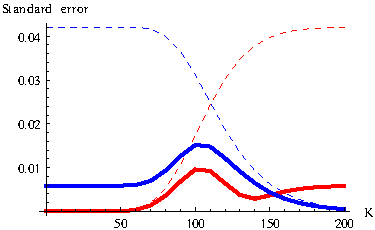
\includegraphics[width=0.4\textwidth]{strike_anti.pdf}}
  \subfloat{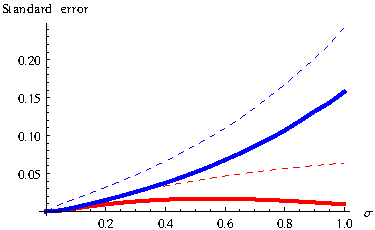
\includegraphics[width=0.4\textwidth]{vol_anti.pdf}}
  \caption{The put (red) and call (blue) option price errors as a function of $K$ (left figure) and $\sigma$ (right figure). The dashed lines are the errors without the use of antithetic variables.}
  \label{fig:anti}
\end{figure}

The figures show some irregular behavior compared to the model without antithetic variables. When we vary the strike, the error still goes to zero when the option price goes to zero (for the same reason as given in Part I). However, the error has a maximum when the strike price is equal to $S_0$. However for all values of the strike price the error when using antithetic variables is smaller then the original model. The error as a function of $\sigma$ behaves the same way as with the original model, only the errors are significantly smaller for large $\sigma$.

To give an intuitive explanation for the reduction on the standard error we first look at the ideal case of a linear function with antithetic variables. For this function the standard error is always zero, because the positive and negative terms cancel each other out. Now when K is small (for a call) or large (for a put), the maximum is almost always nonzero and the function becomes more like the symmetric case. So the terms cancel each other more out and the variance becomes lower.

When we consider the standard error as a function of $\sigma$ we also see an improvement with the use of antithetic variables. This is because the payoff is somewhat linear. Just as we saw in the other graph: the more linear the function the better antithetic variables work. Note that for the put the error goes to zero. This is because the sigma term becomes dominant. As a result $S_T=S_0e^{(r-1/2\sigma^2)T+\sigma\sqrt{T}Z}$ will become lower and the payoff of a put goes to zero.

We also investigate the behavior of an Asian option, modeled with Monte Carlo and antithetic variables, as described in the previous section. We evaluate the stock price daily and take a maturity of one year (assuming 365 business days). We first look at the behavior of the Asian option price for $K = 99, S_0 = 100, r = 0.06$ and $\sigma = 0.20$ where we take different sample sizes ($M = 10^{5..7}$). The results are given in table \ref{tab:asian} below.

\begin{table}[H]
  \centering
  \begin{tabular}{l || c }
    \hline
    M & Asian price \\
    \hline
    $10^5$ & 6.588809 $\pm$ 0.025091 \\
    $10^6$ & 6.566661 $\pm$ 0.007887 \\
    $10^7$ & 6.561250 $\pm$ 0.002495 \\
  \end{tabular}
  \caption{Results for the Asian call option with error.}
  \label{tab:asian}
\end{table}

As we see here, the error is getting closer to zero as the sample size increases. We will later compare this value with the analytical value of an Asian option with a geometric average, which can be solved analytically.

Furthermore we also look at the behavior of the Asian option price as a function of $K$ ($r = 0.06, \sigma = 0.20, S_0 = 100, M = 10^6$). The figure \ref{fig:asianstrike} below shows the option price as a function of $K$ (left) as well as the error on the option price as a function of $K$. We observe a linear decrease in the option price if $K < S_0$, which is caused by the payoff, which increases linearly with decreasing $K$, since the option behaves similarly to an European call option. Furthermore we observe an error which is large around $K = S_0$, similar to what we found for the European call/put option with antithetic variables. We observe again that the error goes to zero when the option price goes to zero. When $K$ is small enough, the error is constant, because of the disappearance of the zeros, as we observed also in part I of the assignment (the normal distribution of the payoff is not compressed anymore and just shifts with decreasing $K$).

\begin{figure}[H]
  \centering
  \subfloat{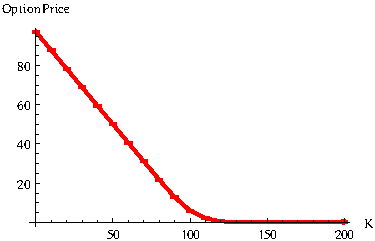
\includegraphics[width=0.4\textwidth]{asianstrike.pdf}}
  \subfloat{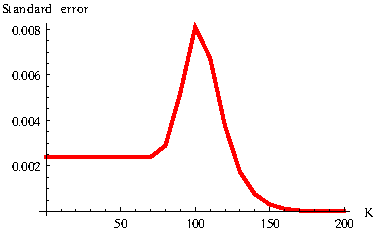
\includegraphics[width=0.4\textwidth]{asianstrikeerror.pdf}}
  \caption{The Asian option price as a function of $K$ (left) and the standard error as a function of $K$ (right). This model uses antithetic variables.}
  \label{fig:asianstrike}
\end{figure}

Lastly we also looked at the behavior of the option price as a function of $\sigma$ ($r = 0.06, K = 99, S_0 = 100, M = 10^6$). The figure \ref{fig:asianvol} below shows the option price as a function of $\sigma$ (left) as well as the error as a function of $\sigma$ (right). We see that the option price increases in the same way as in the case of the European call for increasing $\sigma$ with an offset at $\left(\frac{100*\text{exp}(0.06)+100}{2} - 99\right)*\text{exp}(0-0.06) = 3.85$. This is because of the same reasons as before, an increase in volatility increases the price as the payoff increases with increasing $\sigma$, while the loss is not large because the option is not exercised in that case. We also see that the error (right figure) behaves similarly compared with the European call option. Overall the behavior of the Asian call option is very similar to that of an European call option.

\begin{figure}[H]
  \centering
  \subfloat{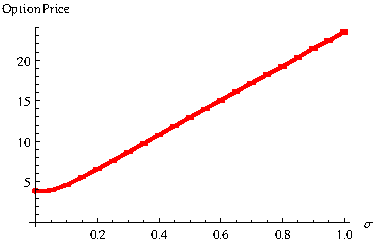
\includegraphics[width=0.4\textwidth]{asianvol.pdf}}
  \subfloat{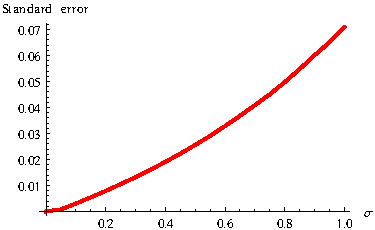
\includegraphics[width=0.4\textwidth]{asianvolerror.pdf}}
  \caption{The Asian option price as a function of $\sigma$ (left) and the standard error as a function of $\sigma$ (right). This model uses antithetic variables.}
  \label{fig:asianvol}
\end{figure}

\subsection{Part B: Control Variates}

\subsubsection{Theory}
We start with the explanation of the use of control variates. This explanation is a rephrasing of the explanation given in \cite{ross}. We want to estimate $\theta=\mathbb{E}[X]$ where $X$ is the output of our simulation. Now suppose that we have some other output variable $Y$, the expected value of $Y$ is known, $\mathbb{E}[Y]=\mu_y$. For this technique to work $\text{Var}(Y)$ has to be bigger then zero. Then for any constant $c$, the estimator

\begin{equation}
\label{eq:controlvariate}
T=X+c(Y-\mu_y)
\end{equation}

is also an unbiased estimator of $\theta$. Now we have some freedom to choose $c$, and we are going to choose $c=c^*$, such that the variance of the new estimator is minimized. Note that

\begin{align}
\text{Var}(T)=\text{Var}(X+c(Y-\mu_y))&=\text{Var}(X+c(Y))\\
&=\text{Var}(Y)c^2+2\text{Cov}(X,Y)c+\text{Var}(X)
\end{align}

This is always a parabola with a minimum, since $\text{Var}(Y)>0$. With the ABC-formula we find the symmetry point, also the minimum $c^*$. So

\begin{equation}
c^*=-\frac{\text{Cov(X,Y)}}{\text{Var}(Y)}
\end{equation}

With this value our estimator becomes
\begin{equation}
T=X-\frac{\text{Cov}(X,Y)}{\text{Var}Y}(Y-\mu_Y)
\end{equation}
This estimator has a variance
\begin{equation}
\text{Var}(T)=\text{Var}(X+c^*(Y-\mu_Y))=\text{Var}(X)-\frac{\text{Cov}(X,Y)^2}{\text{Var}(Y)}
\end{equation}

It is important to realize that $\text{Var}X\geq\text{Var}T$ since $\frac{\text{Cov}(X,Y)^2}{\text{Var}(Y)}$ is always a positive term. So we the estimator works best when the $Y$ ($Y$ is called the control variate) is heavily correlated with X.

Since we want to apply this technique to an Asian call option based on arithmetic averages, we now proceed with deriving an expression for the price of an Asian option that is based on geometric averages. We recall that the geometric average is defined as

\begin{equation}
\label{eq:as}
\widetilde{A}_N=\left(\prod_{i=1}^N S_i\right)^{\frac{1}{N}}
\end{equation}

Just as in the derivation of a call option price, we look at the logarithm of the underlying. Since the logarithm of the geometric average has just as the stock price a normal distribution. We will derive the distribution of 

\begin{equation}
\log\frac{\left(\prod_{i=1}^N S_i\right)^{\frac{1}{N}}}{S_0}
\end{equation}

We want to split this expression up in different independent increments, because we know the sum of two independent normally distributed random variables. We rewrite the expression into a telescopic sum and simplify the expression

\begin{align}
\log\frac{\left(\prod_{i=1}^N S_i\right)^{\frac{1}{N}}}{S_0}&=\frac{1}{N}\log\left(\left(\frac{S_1}{S_0}\right)^N\left(\frac{S_2}{S_1}\right)^{N-1}\cdots\frac{S_N}{S_{N-1}}\right)\\
&=\frac{1}{N}(\log S_1-\log S_0)+\frac{2}{N}(\log S_2- \log S_1)+\ldots+\frac{N}{N}(\log S_N-\log S_{N-1})
\end{align}

From assignment 1 we recall that $\log(S(t_2)-S(t_1))\sim\mathcal{N}((r-1/2\sigma^2)(t_2-t_1),\sigma^2(t_2-t_1))$ for any $0<t_1<t_2<T$ (with the $\mathcal{N}(\mu,\sigma^2)$ notation). Thus we know that each increment of the logarithm of a stock is normally distributed with mean $(r-1/2\sigma^2)\Delta t$ and variance $\sigma^2 \Delta t$. 

\begin{equation}
\log\frac{\left(\prod_{i=1}^N S_i\right)^{\frac{1}{N}}}{S_0}\sim \frac{1}{N}\mathcal{N}((r-\tfrac{1}{2}\sigma^2)\Delta t,\sigma^2 \Delta t)+\frac{2}{N}\mathcal{N}((r-\tfrac{1}{2}\sigma^2)\Delta t,\sigma^2 \Delta t)+\ldots+\frac{N}{N}\mathcal{N}((r-\tfrac{1}{2}\sigma^2)\Delta t,\sigma^2 \Delta t)
\end{equation}

Furthermore the increments are non overlapping and thus independent. So we can use the rule for the sum of two independent normal distributions $a\mathcal{N}(\mu_1,\sigma_1^2)+b\mathcal{N}(\mu_2,\sigma_2^2)=\mathcal{N}(a\mu_1+b\mu_2,a^2\sigma_1^2+b^2\sigma_2^2)$. This brings us to

\begin{equation}
\log\frac{\left(\prod_{i=1}^N S_i\right)^{\frac{1}{N}}}{S_0}\sim\mathcal{N}\left((r-\tfrac{1}{2}\sigma^2)\Delta t\frac{1}{N}(1+2+\ldots+N),\sigma^2 \Delta t \frac{1}{N^2}(1+2^2+\ldots+N^2)\right)
\end{equation}

Where we know that $1+2+\ldots+N=\frac{N(N+1)}{2}$ and $1+2^2+\ldots+N^2=\frac{N(N+1)(2N+1)}{6}$. Filling them in and using $\Delta t=\frac{T}{N}$ gives the desired expression:

\begin{equation}
\log \frac{\widetilde{A}_N}{S_0}=\log\frac{\left(\prod_{i=1}^N S_i\right)^{\frac{1}{N}}}{S_0}\sim\mathcal{N}\left((r-\tfrac{1}{2}\sigma^2)\frac{N+1}{2N}T,\sigma^2 \frac{(N+1)(2N+1)}{6N^2}T\right)
\end{equation}

To determine the price of an Asian option based on geometric averages at time zero we want to calculate $\tilde{a}=e^{-rT}\mathbb{E}\left[(\widetilde{A}_N-K,0)^+\right]$. We can do this on a similar way as in the Black-Scholes case for an European call option. For the discounting to make sense we have to rewrite the underlying. Let $\widetilde{A}_N=\widetilde{S}_T$, such that

\begin{equation}
\log \frac{\widetilde{A}_N}{S_0}=\log \widetilde{S}_T-\log S_0\sim\mathcal{N}((\tilde{r}-\tfrac{1}{2}\tilde{\sigma}^2)T,\tilde{\sigma}^2T)
\end{equation}

with $\tilde{\sigma}=\sigma\sqrt{\frac{(N+1)(2N+1)}{6N^2}}$ and $\tilde{r}=(r-\tfrac{1}{2}\sigma^2)\frac{N+1}{2N}+\tfrac{1}{2}\tilde{\sigma}^2$.

For this underlying we have obtained an analytical price in the first assignment, namely:
\begin{equation}
\tilde{c}=e^{-\tilde{r}T}\mathbb{E}\left[(\widetilde{S}_T-K,0)^+\right]=S_0\mathcal{N}(\tilde{d}_1)-Ke^{-rT}\mathcal{N}(\tilde{d}_2)
\end{equation}

where $\tilde{d}_1=\frac{\log\left(\frac{S_0}{K}\right)+\left(\tilde{r}+\frac{1}{2}\tilde{\sigma}^2\right)T}{\tilde{\sigma}\sqrt{T}}$ and $\tilde{d}_2=\tilde{d}_1-\tilde{\sigma}\sqrt{T}$. With a little algebra we get:

\begin{equation}
\label{eq:asiangeom}
\tilde{a}=e^{(\tilde{r}-r)T}\tilde{c}=e^{(\tilde{r}-r)T}(S_0\mathcal{N}(\tilde{d}_1)-Ke^{-\tilde{r}T}\mathcal{N}(\tilde{d}_2))
\end{equation}

\subsubsection{Method}
We apply control variates to do a Monte Carlo simulation for the price of an Asian option based on the arithmetic average. We take as control variate the geometric average, from which we know the analytic solution, namely equation \ref{eq:asiangeom}. We start by estimating the value of $c^*$, as described in the theory above. To this end we first simulate $10^4$ Monte Carlo paths and calculate the geometric and arithmetic option payoffs. From this we can calculate the covariance between these, giving by:

\begin{equation}
  \text{Cov}(\text{geom.},\text{arith.}) = \mathbb{E}[\text{geom.}*\text{arith.}] - \mathbb{E}[\text{geom.}]\mathbb{E}[\text{arith.}]
\end{equation}

and we also calculate the variance on the geometric payoff. With these values we can approximate the optimal value $c^*$. After determining $c^*$ we run our normal Monte Carlo simulation for the geometric average, but the payoff we compute is now given according by equation \ref{eq:controlvariate}:

\begin{equation}
  \text{payoff} = \text{arith.} - c^*(\text{geom.} - \mu_{\text{geom.}})
\end{equation}

where $\mu_{\text{geom.}}$ is given by equation \ref{eq:asiangeom} and multiplied by $e^{r}$ since we are considering the payoff here, and equation \ref{eq:asiangeom} is the discounted value of the payoff. We still only use one random number per sample, since the geometric and arithmetic averages are calculated over the same stock price series. We can calculate the variance on the payoff as given in the equation above, which should be significantly reduced. Note that this method is fairly slow in execution, since we have to calculate for each Monte Carlo run the arithmetic and the geometric average, which is about 50\% more work as just calculating the arithmetic average.

Furthermore the calculation of the geometric average has some problems when implemented in C, since the amount that needs to be calculated is roughly $100^{365}$ which exceeds the data type size of a (long) double. A possible solution would be to get the power in to the sum (equation \ref{eq:as}), this causes however rounding errors which behave unpredictable since the rounding errors are multiplied. The method we choose to implement this relatively safely is by taking the log of equation \ref{eq:as} and after the arithmetic average is computed, taking the exponent again. This is however an expensive operation, since the log of the stock price has to be calculated at every time step.

\subsubsection{Results}
We first validate our model by comparing the results for the Asian option with the results given in Part A of the third part of the assignment. Therefore we calculate the arithmetic Asian option price with the geometric price as a control variate with $S_0 = 100, K = 99, \sigma = 0.20$ and $r = 0.06$. We first performed a small simulation consisting of $10^4$ paths to estimate a value for $c^*$, which was found to be $-1.038408$. The analytical price for the geometric Asian option for these parameters is $6.331828$. We then proceed by calculating the estimate of the arithmetic Asian option price, the results are given in the table below, together with the values also reported in table \ref{tab:asian}:

\begin{table}[H]
  \centering
  \begin{tabular}{l || c | c }
    \hline
    M & Asian price (with antith. var.) & Asian price (with contr. var.) \\
    \hline
    $10^5$ & 6.588809 $\pm$ 0.025091 & 6.566295 $\pm$ 0.001528\\
    $10^6$ & 6.566661 $\pm$ 0.007887 & 6.565699 $\pm$ 0.000487\\
    $10^7$ & 6.561250 $\pm$ 0.002495 & 6.565547 $\pm$ 0.000152\\
  \end{tabular}
  \caption{Results for the Asian option with error, both with antithetic variables and the control variate.}
  \label{tab:asian}
\end{table}

From the table we can conclude that the control variate technique greatly reduces the variance, while both the values are still in each others range when taking into account the errors. 

We can also investigate the behavior of the error as a function of $K$ and $\sigma$ as we did before with $M = 10^6$ and the default values for the other parameters. Since the price is the same as the price calculated in part A for the Asian option, we do not plot the prices here. The errors for $K$ and $\sigma$ are given in figure \ref{fig:asianvar} below, left for $K$ and right for $\sigma$. The dotted lines are the errors in the case of the use of antithetic variables, the solid lines are the results for the control variate method.

\begin{figure}[H]
  \centering
  \subfloat{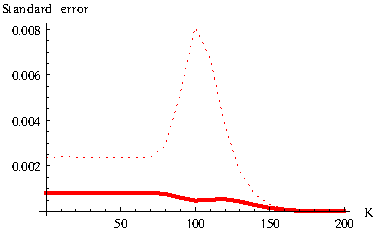
\includegraphics[width=0.4\textwidth]{asianstrikevar.pdf}}
  \subfloat{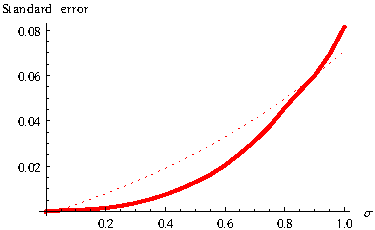
\includegraphics[width=0.4\textwidth]{asianvolvar.pdf}}
  \caption{The error of the Asian option as a function of $K$ (left) and as a function of $\sigma$ (right). The dotted lines are the errors in the case of antithetic variables, the solid lines are for the control variate method.}
  \label{fig:asianvar}
\end{figure}

If we look at the error as a function of $K$ we see that the control variate technique gives better performance than the antithetic variable technique. The spike around $S_0 \approx K$ which occurred for the antithetic variable technique has completely disappeared, there is even a small dip now at this value. If we look at the behavior as a function of $\sigma$ we see that the error has a stronger curvature for the control variate case. The error is even larger than the antithetic variable error for large values of $\sigma$, however these values are so large that they are unrealistic in most of the real world applications. It is interesting to note though that the antithetic method is much faster, since it requires only half the samples, whereas the control variate technique requires almost twice the number of samples, one sample for the geometric average and one for the arithmetic average (although they are sampled with the same random number). In order to determine which one is better to use one should take into account this difference in execution time, for instance when $K$ is small it might be much more profitable to use the antithetic variable method, even though it produces a larger error.

\newpage

\section{Appendix}
\subsection{Derivation of the variance of the payoff}

The variance of the option price is given by:

\begin{equation}
  \text{Var}(e^{-rT}\text{payoff}) = (\mathbb{E}[e^{-rT}\text{payoff}^2] - \mathbb{E}[e^{-rT}\text{payoff}]^2)
\end{equation}

where we know that $\mathbb{E}[e^{-rT}\text{payoff}] = S_0\mathcal{N}(d_1) - Ke^{-rT}\mathcal{N}(d_2)$ with $d_1 = \frac{log(\frac{S_0}{K}) + (r + 0.5\sigma^2)T}{\sigma \sqrt{T}}$ and $d_2 = d_1 - \sigma \sqrt{T}$, which is the Black Scholes formula. We can derive an expression similar to Black Scholes for the quadratic payoff, first noting that:

\begin{align}
  &\mathbb{E}[e^{-rT}\text{payoff}^2] = e^{-rT}\mathbb{E}[\text{max}(S_T-K,0)^2] \nonumber \\
  & = e^{-rT}\mathbb{E}[\text{max}((S_T-K)^2,0)] \nonumber \\
  & = e^{-rT}\mathbb{E}[\text{max}((e^{x_T \hat{\sigma} + \hat{\mu}} - K)^2,0)]
\end{align}

where $x_T = \frac{\text{log}(S_T) - \hat{\mu}}{\hat{\sigma}}$ with $S_T$ distributed according to equation \ref{eq:st}, $\hat{\mu} = (r - 0.5\sigma^2)T + \text{log}(S_0)$ and $\hat{\sigma} = \sigma \sqrt{T}$. From this it follows that $x_T ~ \mathcal{N}(0,1)$ with standard normal distribution $\phi(x_T)$. We can now further evaluate the expectation:

\begin{align}
  &e^{-rT}\mathbb{E}[\text{max}((e^{x_T \hat{\sigma} + \hat{\mu}} - K)^2,0)] \nonumber \\
  & = e^{-rT}\int_{\frac{\log K -\hat{\mu}}{\hat{\sigma}}}^{\infty}{(e^{x_T\hat{\sigma}+\hat{\mu}}-K)^2\phi(x_T)}\mathrm{d}x_T \nonumber \\
  & = e^{-rT}\int_{\frac{\log K -\hat{\mu}}{\hat{\sigma}}}^{\infty}{(e^{2(x_T\hat{\sigma}+\hat{\mu})}-2Ke^{(x_T\hat{\sigma}+\hat{\mu})}+K^2)\phi(x_T)}\mathrm{d}x_T \nonumber \\
  & = e^{-rT}\int_{\frac{\log K -\hat{\mu}}{\hat{\sigma}}}^{\infty}{e^{2(x_T\hat{\sigma}+\hat{\mu})}\phi(x_T)}\mathrm{d}x_T +
  e^{-rT}\int_{\frac{\log K -\hat{\mu}}{\hat{\sigma}}}^{\infty}{-2Ke^{(x_T\hat{\sigma}+\hat{\mu})}\phi(x_T)}\mathrm{d}x_T + \nonumber \\
  & e^{-rT}\int_{\frac{\log K -\hat{\mu}}{\hat{\sigma}}}^{\infty}{K^2\phi(x_T)}\mathrm{d}x_T
\end{align}

From the derivation of Black-Scholes in the last assignment, we can immediately give the results for the last two terms, since they are similar to the ones in the Black-Scholes derivation, just with different factors in front (for details, please see the report of assignment 1).

\begin{align}
  e^{-rT}\int_{\frac{\log K -\hat{\mu}}{\hat{\sigma}}}^{\infty}{-2Ke^{(x_T\hat{\sigma}+\hat{\mu})}\phi(x_T)}\mathrm{d}x_T &\rightarrow -2KS_0\mathcal{N}(d_1) \nonumber \\
  e^{-rT}\int_{\frac{\log K -\hat{\mu}}{\hat{\sigma}}}^{\infty}{K^2\phi(x_T)}\mathrm{d}x_T &\rightarrow K^2e^{-rT}\mathcal{N}(d_2)
\end{align}

For the first term we also use an approach similar to the one used for the evaluation of the first integral above. We first rewrite the integrand:

\begin{align}
  &e^{2x_T\hat{\sigma}+2\hat{\mu}}\phi(x) \nonumber \\
  & =\frac{1}{\sqrt{2\pi}}e^{-\frac{x^2-4x\hat{\sigma}-4\hat{\mu}}{2}} \nonumber \\
  & =\frac{1}{\sqrt{2\pi}}e^{-\frac{(x-2\hat{\sigma})^2-2\hat{\mu}-4\hat{\sigma}^2}{2}} \nonumber \\
  & =e^{2\hat{\mu}+2\hat{\sigma^2}}\phi(x-2\hat{\sigma})  
\end{align}

Implementing this with $1-\mathcal{N}(x)=\mathcal{N}(-x)$ yields:

\begin{align}
&e^{-rT}\int_{\frac{\log K -\hat{\mu}}{\hat{\sigma}}}^{\infty}{e^{2\hat{\mu}+2\hat{\sigma^2}}\phi(x-2\hat{\sigma})}\mathrm{d}x \nonumber \\
& = e^{-rT+2\hat{\mu}+2\hat{\sigma^2}}\left(1-\mathcal{N}\left(\frac{\log K -\hat{\mu}}{\hat{\sigma}}-2\hat{\sigma}\right)\right) \nonumber \\
& = e^{-rT+2\left(r-\frac{1}{2}\sigma^2\right)T+2\sigma^2T+2\log S_0}\left(\mathcal{N}\left(\frac{-\log K +\hat{\mu}}{\hat{\sigma}}+2\hat{\sigma}\right)\right) \nonumber \\
& = S_0^2e^{rT+\sigma^2T}\mathcal{N}\left(\frac{\log\left(\frac{S_0}{K}\right)+\left(r-\frac{1}{2}\sigma^2\right)T}{\sigma\sqrt{T}}+2\sigma\sqrt{T}\right) \nonumber \\
& = S_0^2e^{rT+\sigma^2T}\mathcal{N}(d_1+\sigma \sqrt{T})
\end{align}

All together we obtain the following expression for the variance on the option price, $\text{Var}(e^{-rT}\text{payoff})$:

\begin{align}
  \label{eq:var}
  \text{Var}(e^{-rT}\text{payoff}) =& K^2e^{-rT}\mathcal{N}(d_2)-2KS_0\mathcal{N}(d_1) + S_0^2e^{rT+\sigma^2T}\mathcal{N}(d_1+\sigma \sqrt{T}) \nonumber \\
  &-(S_0\mathcal{N}(d_1) - Ke^{-rT}\mathcal{N}(d_2))^2 
\end{align}

from which we can calculate the standard deviation by taking the square root, and the standard error with 95\% confidence intervals by dividing by the square root of the sample number and multiplying by 1.96.

\subsection{The $\delta$ of a digital call option}
Using the Black-Scholes model it is easy to derive an expression for the payoff of a digital option; simply put in the (simpler) function $I(S_T > K)$ instead of $\text{max}(S_T - K, 0)$ and repeat the calculations. For details of the Black-Scholes model see the previous assignment. Using this derivation the price for a digital call option is given by:

\begin{equation}
  C = e^{-rT}\mathcal{N}(d_2)
\end{equation}

with $d_1 = \frac{log(\frac{S_0}{K}) + (r + 0.5\sigma^2)T}{\sigma \sqrt{T}}$ and $d_2 = d_1 - \sigma \sqrt{T}$. Within the Black-Scholes model, $\delta = \frac{\partial C}{\partial S}$ and hence:

\begin{equation}
  \label{eq:deltadigital}
  \delta = \frac{\partial C}{\partial S} = \frac{e^{-rT}\mathcal{N}'(d_2)}{\sigma S \sqrt{T}}
\end{equation}

where $\mathcal{N}'(d_2)$ is given by differentiating the integral of the normal distribution:

\begin{equation}
  \mathcal{N}'(d_2) = \frac{1}{\sqrt{2\pi}} \exp{(-0.5d_2^2)}
\end{equation}

If we take $T = 1, K = 99, S_0 = 100, r = 0.06$ and $\sigma = 0.20$ we can calculate the value of $\delta$ at time 0, which is approximately 0.018206. This is the value which is used for comparison in table \ref{tab:deltadigital} and table \ref{tab:likelihood}.

\begin{thebibliography}{10}
\bibitem{boxmuller} 
  G.E.P. Box, M.E. Muller, \emph{A Note on the Generation of Random Normal Deviates}, The Annals of Mathematical Statistics, 1958, Vol. 29, No. 2, 610-611
\bibitem{heath}
  M.T. Heath, \emph{Scientific Computing: An Introductory Survey, 2nd Ed.}, McGraw Hill, 2005
\bibitem{ross}
  S.M. Ross, \emph{Simulation, 4th Ed.}, Academic Press, 2006
\bibitem{Glasserman}
  P.Glasserman, \emph{Monte Carlo methods in financial engineering}, Springer, 2004. 
\bibitem{savickas}
  V. Savickas, \emph{Fast Greeks: Case of Credit Valuation}, MSc Thesis 2011, Utrecht University.
\end{thebibliography}

\end{document}
